\documentclass[conf]{new-aiaa}

\usepackage{float}
\usepackage{subfigure}
\usepackage[justification=centering]{caption}
\usepackage{multirow} \usepackage{graphicx}
  \graphicspath{ {./images/} }
\usepackage{nameref}
\usepackage{amsmath}
\usepackage{amssymb}
\usepackage{amsfonts}
\usepackage[linesnumbered,ruled]{algorithm2e}
\usepackage{tikz}
\usetikzlibrary{calc,patterns,decorations.pathmorphing,decorations.markings,positioning,automata,shapes,arrows}
  \tikzstyle{block} = [rectangle, draw, text width=3.5cm]
  \tikzstyle{line} = [draw, -latex']
\usepackage{pgfplots}
  \pgfplotsset{compat=1.3}
\usepgfplotslibrary{colormaps,external}
\usepackage{ulem}
\usepackage{verbatim}
\usepackage[version=4]{mhchem}
\usepackage{siunitx}
\usepackage[super]{nth}
\usepackage{pbox}
\usepackage{longtable,tabularx}
  \setlength\LTleft{0pt} 

\title{ Deformation of a Panel in Repeated High Speed Flow 
        Modeled with Creep and Multiplicatively-Decomposed Plasticity}

\author{Justin L. Clough%
        \footnote{
          PhD Student, 
          justin.clough1@gmail.com,
          Aerospace and Mechanical Engineering Department, 
          854 Downey Way, RRB 101,
          Student Member}
        and Assad A. Oberai%
        \footnote{  
          Professor, 
          Aerospace and Mechanical Engineering Department, 
          854 Downey Way, RRB 101.}}
\affil{University of Southern California,
       Los Angeles, CA, 90089}

\author{Jos\'e A. Camberos%
        \footnote{
          Team Lead of Design of Aerospace Systems for Hypersonics, 
          Air Force Research Laboratory,
          Wright-Patterson AFB, OH 45433,
          Associate Fellow.
          \newline
          \newline
          Previous version submitted as extended abstract:
            \sout{DISTRIBUTION A. Approved for public release: distribution unlimited. 
            Cleared under number 88ABW-2019-4012.}}} 
\affil{Air Force Research Laboratory, Wright-Patterson AFB,
       Dayton, OH, 45433}


\begin{document}
\maketitle

\begin{abstract} %TODO: Update from abstract submission to full paper submission
The surface skin panels of high speed vehicles can reach high 
temperatures when in flight. 
These temperatures are greater than the solidus temperature
of aluminum alloys and in the range where
creep has been observed for titanium alloys.
Studies have modeled the permanent set and deformation 
of panels using small strain plasticity.
They have also accounted for temperature
dependent material properties in their constitutive models.
This work models the creep of a stiffened panel
from a conceptual high speed vehicle.
A titanium alloy, Ti6Al4V,
is used as it is common in the design of high speed vehicles.
Multiplicatively-decomposed plasticity 
is included in the constitutive law as well to allow for large strains.
The panel geometry from a high speed concept vehicle is
used with boundary conditions to induce thermal buckling.
A uniform temperature is prescribed on the panel
based on recent measurements.
The temperature is cycled to simulate phases of
heating, cruise, and cooling over multiple flights.
Preliminary analytical work considered a single strip
of vehicle paneling under two flight cycles.
The results show that the creep strain
grew to within 98\% of those induced by thermal strains 
over two representative flight cycles.
\end{abstract}

%-----------------------------------------------------------------------------%
\section{Nomenclature} %TODO: Update from abstract submission to full paper submission

{\renewcommand\arraystretch{1.0}
\noindent\begin{longtable*}{@{}l @{\quad=\quad} l@{}}
$\bar{A}$    & Relaxation rate\\
$c_1$        & Stress Exponent\\
$E$          & Young's Modulus \\
$F$          & Deformation gradient\\
$J$          & Ratio of volumetric change\\
Ma           & Mach number\\
$Q$          & Activation energy\\
$R$          & Universal gas constant\\
$t$          & Time\\
$t_{ss}$     & Steady state time\\
$t_{f}$      & Flight time \\
$\alpha$     & Coefficient of thermal expansion\\
$\epsilon^T$ & Total strain\\
$\epsilon^e$ & Elastic strain\\
$\epsilon^c$ & Creep strain\\
$\sigma$     & Cauchy stress\\
$\sigma_0$   & Reference stress\\
$\tau$       & Kirchhoff stress\\
$\theta$     & Temperature\\
$\theta_0$   & Initial temperature
\end{longtable*}}

%-----------------------------------------------------------------------------%
\section{Introduction} %TODO: Update from abstract submission to full paper submission
% Outline:
% - Overview of hypersonic structures
%   - Emph: re-usability
% - What is high speed flow? Characteristics
% - When does and doesn't inertia matter?
% - When does large strain matter?
% - What is creep/ Norton creep?

High speed flow over a vehicle creates a harsh environment for 
the vehicle structure.
For example, the skin of the X-15 regularly saw temperatures
as high as 1220 $^{\circ}$F (933 K)
during its flights up to Mach 6.7
\cite{ kordes_structureal_heating_experiencs_on_the_x15_airplane}.
A recent study by Culler et al.
\cite{ culler_impact_of_FTS_coupling_on_response_prediction_hypersonic_skin_panels}
estimated temperatures exceeding 2500 $^\circ$F (1644 K) 
on the skin of a conceptual high speed vehicle.
These temperatures are greater than the solidus 
temperature of typical aluminum alloys used in aircraft design
\cite{ SAE_metals_and_alloys_in_the_unified_numbering_system}
and within the range where creep has been observed for 
high temperature titanium alloys 
\cite{
  evans_effects_of_alpha_case_formation_on_creep_fracture_properties_of_the_high_temperature_titanium_alloy_IMI834,
  lavina_creep_behavior_of_Ti6Al4V_from_450C_to_600C}.

The skin of a high speed vehicle must support both
the aerodynamic tractions and heating during flight.
Recent interest in reusable vehicles requires
the skin to endure multiple cycles of this loading
\cite{
  walker_falcon_htv_3X_a_resuable_hypersonic_test_bed,
  eason_structures_perspective_on_the_challenges_associated_with_analyzing_reuasble_hypersonic_platform,
  zuchowski_AVIATR_Predictive_capability_for_hypersonic_structural_response_and_life_prediction_phase_II,
  lafontaine_effects_of_strain_hardeing_on_response_of_skin_panels_in_hypersonic_flow}.
The skin panels are typically designed as thin face plates supported 
by stiffeners 
\cite{
  mcnamara_aeroelastic_and_aerothermoelastic_analysis_in_hypersonic_flow_past_present_and_future}.
The face plate and stiffeners of the panel 
can be made of materials that are on the order
of hundredth of an inch thick
\cite{
  plews_a_two_scale_generalized_finite_element_approach_for_modeling_localized_thermoplasticity,
  zuchowski_AVIATR_Predictive_capability_for_hypersonic_structural_response_and_life_prediction_phase_II}.
The panels are compliant and can exhibit combinations of
inertia dominated flapping or thermally induced buckling
\cite{
  thornton_coupled_flow_thermal_and_structural_analysis_of_aerodynamically_heated_panels,
  mei_review_of_nonlinear_panel_flutter_at_supersonic_and_hypersonic_speeds}.
Much work has been done to investigate the fluttering 
of panels in high speed flow
\cite{
  mcnamara_aeroelastic_and_aerothermoelastic_analysis_in_hypersonic_flow_past_present_and_future,
  riley_interaction_between_aerothermally_compliant_structures_and_boudnary_layer_transition_in_hypersonic_flow,
  spottswood_exploring_the_response_of_a_thin_flexible_panel,
  savino_aerothermodynamic_study_of_ultrahigh_termperature_cermaic_winglet_for_atmospheric_reentry_test,
  nydick_hypersonic_panel_flutter_studies_on_cruved_panels,
  lafontaine_effects_of_strain_hardeing_on_response_of_skin_panels_in_hypersonic_flow}.


A study by LaFontaine et al.
\cite{
  lafontaine_effects_of_strain_hardeing_on_response_of_skin_panels_in_hypersonic_flow}
investigated the effects of accumulated 
plastic strain and permanent set of a panel in high speed flow.
The panel material in this study was modeled with an additive 
strain decomposition, a Chaboche kinematic hardening model,
and a $J_2$ flow rule. 
The panel interaction with the flow was modeled through
Eckert's reference enthalpy method 
\cite{
  eckert_engineering_relations_for_heat_transfer_and_friction_in_high_velocity_laminar_and_turbulent_flow}
and \nth{3} order piston theory
\cite{
  meijer_generalized_formulation_and_review_of_piston_theory_for_airfoils}.
The study found that by including plasticity, 
the behavior of the panel changed after four loading cycles 
as compared to an otherwise equivalent linearly elastic panel;
each cycle represented one ten second flight.
Both the elastic and plastic panel originally showed a mix of 
aeroelastic flutter with periods of thermal buckling. 
After the third cycle, the plastic panel demonstrated only thermal
buckling behavior.

This study further investigates the role creep and plasticity play 
in the permanent deformation of a panel under repeated high speed flight.
The amount of deformation of a body undergoes due to creep increases 
with both time and temperature
\cite{roylance_mechanics_of_materials_text}. 
Vehicle flight times are typically estimated on the order
of tens of minutes 
\cite{ 
  kordes_structureal_heating_experiencs_on_the_x15_airplane,
  lafontaine_effects_of_strain_hardeing_on_response_of_skin_panels_in_hypersonic_flow,
  zuchowski_AVIATR_Predictive_capability_for_hypersonic_structural_response_and_life_prediction_phase_II}
which is less than the timescale of hours that creep is 
typically associated with 
\cite{ 
  lavina_creep_behavior_of_Ti6Al4V_from_450C_to_600C,
  evans_effects_of_alpha_case_formation_on_creep_fracture_properties_of_the_high_temperature_titanium_alloy_IMI834,
  roylance_mechanics_of_materials_text}.
However, creep effects have been found to be significant on smaller timescales,
on the order of tens of minutes,
where large temperature fluctuations and gradients are found.
An example of this is in flip-chip manufacturing 
where silicon chips undergo a 150 K temperature change 
in 15 minutes
\cite{ 
  li_simulation_of_finite_strain_inelastic_phenomena_governed_by_creep_and_plasticity}.
In this study, plasticity through a von Mises yield surface is also modeled;
a multiplicatively decomposed version is used to allow for 
possible large strains.
The details of the model and implementation used are
discussed in 
\cite{ li_simulation_of_finite_strain_inelastic_phenomena_governed_by_creep_and_plasticity}.
This extended abstract considers the creep strain of a one dimensional bar
representing a strip of vehicle paneling.
A uniform temperature is prescribed with heating rates and saturation 
temperature based on recent literature estimates.
\newline
\newline
\noindent
\emph{Note to the reviewers:} A more extensive review of the 
state of the art will be included in the 
final manuscript.

%-----------------------------------------------------------------------------%
\section{Methods} \label{sec_methods} 

The end goal of this study is to model the large creep deformation of a canonical acreage
panel due to the thermal loads experienced from repeated high speed flight.
Each flight consisting of heating, cruising, and cooling phases, in that order.
The full constitutive law used is presented in the next subsection.
A simplified version of this material model is then used
is a one dimensional example in subsection after that. 
First, the balance of linear momentum without inertial terms is taken as:

\begin{equation}
  \nabla \cdot P + \rho_0 B = 0
\end{equation}

\noindent
where $P$ is the first Piola-Kirchhoff stress, 
$\rho_0$ is the density of the material, 
and
$B$ represents all body forces.
This relation holds for all points in the body $\mathcal{B}$.
The first Piola-Kirchhoff stress is related to 
the Cauchy stress, $\sigma$, through:

\begin{equation}
  P = J \sigma F^{-T}
\end{equation}

\noindent
where $F$ is the deformation gradient and
$J$ is its Jacobian; $J=\det(F)$.
Additionally, on the boundaries of $\mathcal{B}$:

\begin{align}
  P \cdot N &= \bar{t^{N}} \text{ on } \partial_t \mathcal{B} \\
          u &= \bar{u}     \text{ on } \partial_u \mathcal{B} 
\end{align}

\noindent
where $N$ is the outward normal on $\partial_t \mathcal{B}$
and the boundaries of $\mathcal{B}$ meet the conditions 
that $\partial_t \mathcal{B} \cap \partial_u \mathcal{B} = \emptyset$
and
$\partial_t \mathcal{B} \cup \partial_u \mathcal{B} = \partial \mathcal{B}$.
The deformation gradient is then split into elastic
and inelastic parts as $F^e$ and $F^i$, respectively.

\begin{equation}
  F = F^e F^i
\end{equation}

\noindent
The Jacobian of the elastic part of the deformation gradient
is then $J^e = \det{ F^e}$. 
With this, the elastic part of the left 
Cauchy-Green tensor is defined as:

\begin{equation}
  \bar{b^e} = J^{e^{\frac{-2}{3}}} F^e F^{e^T}
\end{equation}

\subsection{Constitutive Law}
\noindent
The constitutive law used was first presented by Li, et al. in 
\cite{li_simulation_of_finite_strain_inelastic_phenomena_governed_by_creep_and_plasticity}.
The Kirchhoff stress, $\tau$, which is 
related to the Cauchy stress through $\tau = J \sigma$,
is taken as:

\begin{equation}
  \tau = \left( \frac{\kappa}{2} \left( \frac{J^{e^2} - 1}{J^e} \right) - \beta \Delta \theta \right) + \mu \text{dev}( \bar{b^e})
\end{equation}

\noindent
where $\kappa$ is the bulk modulus, 
$\mu$ is the shear modulus,
$\beta$ is the Coefficient of Thermal Expansion (CTE),
and
$\Delta \theta$ is the change in temperature.
The bulk and shear modulus are related to 
Young's modulus, $E$, and Poisson's ratio, $\nu$, through:

\begin{equation}
  \kappa = \frac{E}{3(1-2\nu)}
\end{equation}

\begin{equation}
  \mu = \frac{E}{2(1+\nu)}
\end{equation}

\noindent
The CTE is related to the linear CTE, $\alpha_L$ through:

\begin{equation}
  \beta = \frac{ E}{ 1-2\nu} \alpha_L
\end{equation}

Next, a yield surface and flow rule are introduced to allow the material 
to deform plastically.
The standard von Mises yield function, or $J_2$ flow theory, is used to 
define the yielding surface:

\begin{equation}
  f(\tau, \alpha) = || \text{dev}(\tau) || - \sqrt{\frac{2}{3}}( \sigma_Y + K \alpha)
\end{equation}

\noindent
where $\alpha$ is the equivalent plastic strain,
$K$ is the hardening modulus,
and $\sigma_Y$ is the yield strength.
Separately, plastic strain rate due to creep is modeled 
through Norton creep:


\begin{equation}
  \dot{\epsilon^c} = \bar{A} e^{\frac{-Q}{R \theta}} \left( \frac{ || \mu \text{dev}(\bar{b^e})||}{\sigma_0} \right)^{c_1} n
\label{eq_norton_creep}
\end{equation}

\noindent
where $\bar{A}$ is the relaxation rate, 
$\sigma_0$ is a reference stress,
$Q$ is the activation energy,
$R$ is the universal gas constant,
$c_1$ is the stress exponent,
and 
$n$ is the unit vector. 
The unit vector represents the direction of strain and is
given by:

\begin{equation}
  n = \frac{\text{dev}( \bar{b^e}) }{ ||\text{dev}( \bar{b^e})||}
\end{equation}

\noindent
Additional support and details are given
in \cite{li_simulation_of_finite_strain_inelastic_phenomena_governed_by_creep_and_plasticity}
to show agreement of this constitutive law  with the second law of thermodynamics.

\subsection{One Dimensional Approximation}
In the analysis below through a simple calculation it is demonstrated
why it is necessary to include the effects of creep plasticity.
As an approximation of the expected creep strain,
a bar that is fixed on both ends is considered as it 
undergoes a relevant temperature history.
This bar represents one strip of skin paneling from 
a high speed vehicle.
The bar starts at temperature $\theta_0$ at a stress free state. 
A uniform temperature $\theta(t)$ is prescribed everywhere.
The total strain within the bar is the sum:

\begin{equation}
\epsilon^T = \epsilon^e  + \epsilon^\theta + \epsilon^c
\label{eq_total_strain_sum}
\end{equation}

\noindent
with $\epsilon^T$ as the total strain,
$\epsilon^e$ as the elastic strain,
$\epsilon^\theta$ as the thermal strain.
A additive decomposition is used here to approximate the multiplicative one 
used in the full constitutive law.
The total deflection, and strain, of the bar must be zero as it 
is fixed on both ends.
Applying this constraint to Eq. \ref{eq_total_strain_sum} gives:

\begin{align}
\epsilon^T &= \epsilon^e + \epsilon^\theta + \epsilon^c = 0 \\
\Rightarrow
  \epsilon^e &= -\left( \epsilon^\theta + \epsilon^c \right)  \label{eq_strain_balance}
\end{align}

\noindent
The stress from temperature change is approximated by
a linear stress-temperature relation. 
The axial component of stress is given as:

\begin{equation}
\sigma = E  \epsilon^e 
\end{equation}

\noindent
where $E$ is Young's Modulus.
Substituting for the strain relation from Eq. \ref{eq_strain_balance} 
and expanding the thermal strain gives:

\begin{align}
\sigma &= -E \left( \epsilon^\theta + \epsilon^c \right)  \\
\sigma &= -E \left( \alpha_L (\theta(t) - \theta_0) + \epsilon^c \right) 
\label{eq_cauchy_stress_sum}
\end{align}

\noindent
Next, it is assumed that there is no volume change over time.
This is consistent with the fixed boundary conditions at 
each end of the bar.
This allows the Kirchhoff stress to be equivalent to the Cauchy stress:

\begin{align}
\tau &= J \sigma \\
\Rightarrow
  \tau &= \sigma \label{eq_cauchy_to_kirchoff}
\end{align}

\noindent
where $J=\det(F)$.
The creep strain rate in one dimension, as outlined in 
\cite{ li_simulation_of_finite_strain_inelastic_phenomena_governed_by_creep_and_plasticity}
and shown in Eq. \ref{eq_norton_creep}, is:

\begin{equation}
\dot{\epsilon^c} = \bar{A} e^{\frac{-Q}{R \theta(t)}} \left( \frac{ ||\tau||}{\sigma_0} \right)^{c_1} \text{sgn}(\tau)
\end{equation}

\noindent
with $\text{sgn}(\cdot)$ as the sign operator to replace the unit vector in the 1D approximation.
Substituting for the Kirchhoff stress from Eq. \ref{eq_cauchy_stress_sum} and \ref{eq_cauchy_to_kirchoff}
then yields the following ODE.

\begin{equation} \label{eq_creep_ode}
\dot{\epsilon^c} = \bar{A} e^{\frac{-Q}{R \theta(t)}} 
    \left( \frac{E || \alpha_L (\theta(t) - \theta_0) + \epsilon^c||}{\sigma_0} \right)^{c_1} 
    \text{sgn}\left( -E \left( \alpha_L (\theta(t) - \theta_0) + \epsilon^c) \right) \right)
\end{equation}

\noindent
The solution to this ODE provides an expression for the creep strain
given a temperature history, $\theta(t)$.


\subsection{Material Properties}
Material properties for titanium alloy Ti6Al4V were estimated from
Lavina et al. \cite{ lavina_creep_behavior_of_Ti6Al4V_from_450C_to_600C}
for creep parameters and from \cite{
boyer_materials_properties_handbook_titanium_alloys}
for the Young's modulus and the linear CTE of the material.
For this unit set the universal gas constant is 8.3145 J/(Mol$\cdot$K)
and the relaxation parameter, $\bar{A}$, was taken as 1 with units of per second.
The material parameters used are shown in Table \ref{tab_material_properties}.

\begin{table}[H]
  \centering
  \caption{
    Material properties used for Ti6Al4V.
    Data from 
    \cite{ lavina_creep_behavior_of_Ti6Al4V_from_450C_to_600C,
      boyer_materials_properties_handbook_titanium_alloys}.}
  \begin{tabular}{|c|c|c|}
    \hline
    Variable & Value & Units  \\
    \hline
    $\sigma_0$ & 22.7  & MPa    \\
    $Q$      & 251     & kJ/Mol \\
    $c_1$    & 12.5    & 1      \\
    $E$      & 113.8   & GPa    \\
    $\alpha_L$ & 9.7E-6  & 1/K    \\
    $\nu$    & 0.33    & 1      \\
    \hline
  \end{tabular}
  \label{tab_material_properties}
\end{table}

\noindent
For reference, a measure of the ``activation temperature'' 
$\left(\frac{Q}{R}\right)$ of Ti6Al4V is 3019 K.

\subsection{Problem Set Up}
The initial and prescribed temperatures are borrowed from 
\cite{ culler_impact_of_FTS_coupling_on_response_prediction_hypersonic_skin_panels}.
In this study, the transient thermo mechanical response of a panel from the 
surface of a representative concept vehicle is simulated with a coupled framework.
The initial temperature is 70 $^{\circ}$F (294 K) and a steady state temperature 
of 2750 $^{\circ}$F (1283 K) is achieved after the first 25 seconds of flight.
Note that the vehicle is assumed to start at its cruising speed of Mach 12
as done in \cite{ culler_impact_of_FTS_coupling_on_response_prediction_hypersonic_skin_panels}.
For the bar approximation, a temperature history with multiple
heating and cooling stages is used.
For the full panel, only the heating portion of flight is considered.
Incorporating this gives $\theta_0 = 294 K$ and:

\begin{equation}
\theta(t) = \begin{cases}
 \theta_0 + (59.65 \text{K/s})t                & t < t_{ss} \\
1783 K                                         & t_{ss} \leq t < t_f-t_{ss} \\
(1783 K) - (59.65 \text{K/s})(t-(t_f-t_{ss}))  & t_f - t_{ss} \leq t
\end{cases}
\end{equation}

\noindent
with $t_{ss}$ as the steady state time of 25 seconds
and $t_f$ representing one flight time.
It was assumed that the steady state time for heating was
equal to that of cooling.
This equates to a linear increase in temperature from 
$\theta_0$ at zero seconds to 1783 K at $t_{ss}$;
this temperature is then held constant until $t_{ss}$ before
the end of the flight.
The temperature then decreases linearly with time back to $\theta_0$.
This is equivalent to a set of heating, cruise, and cooling phases of a single flight.
For both the bar approximation and the full panel, creep is the only
considered method of plasticity; 
a sufficiently high yield strength was used to effectively 
turn off $J_2$ plasticity.

The panel geometry is taken from 
\cite{culler_impact_of_FTS_coupling_on_response_prediction_hypersonic_skin_panels}
and is shown in Figure \ref{fig_panel_face_mesh}.
The mesh is unstructured and populated with composite, 10-node tetrahedral elements.
These elements have been shown to accurately model bending 
without element locking behavior
\cite{ostien_10_node_comp_tet_FE_for_solid_mechanics, 
  clough_automated_wing_internal_structure_placement_guided_by_FEA}.
At least two elements span the thickness of the panel at all locations. 


\begin{figure}[H] 
  \centering
    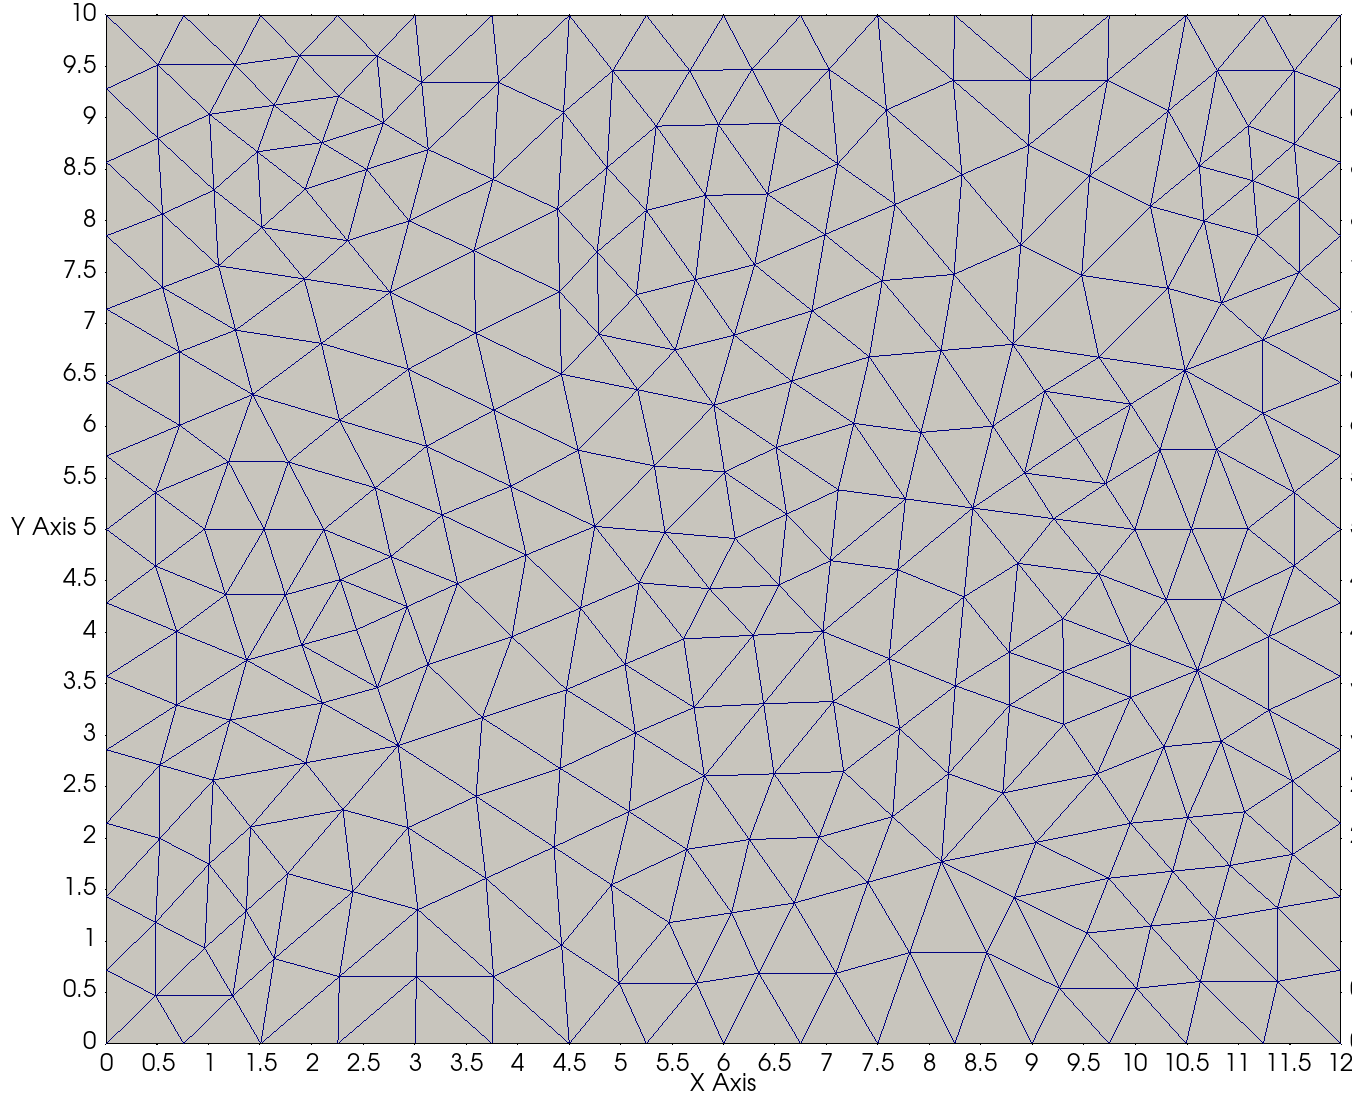
\includegraphics[width=0.35\textwidth, keepaspectratio]
    {panel_face_mesh}
  \caption{ Geometry of the panel with discretization. 
            Panel is approximately 10 in by 12 in and 0.065 in thick
            \cite{culler_impact_of_FTS_coupling_on_response_prediction_hypersonic_skin_panels}.}
  \label{fig_panel_face_mesh}
\end{figure}

\noindent
The panel is fixed in all directions at the left and right most
faces. 
This represents the panel being attached to the substructure of the aircraft
at these locations.
The aforementioned linear temperature change over time is prescribed
uniformly throughout the panel.
Additionally, a uniform pressure is applied to the face of the panel.
This pressure approximates the aerodynamic tractions the 
panel would experience in flight. 
The pressure increases linearly over time from zero to 85.5 KPa. 
This value was chosen as it equals the dynamic pressure
acting on a panel with a $5^{\circ}$ angle of attack
traveling at Mach 12 at an elevation of 104,000 feet above sea level;
these values are consistent with those given
for the conceptual vehicle described in 
\cite{culler_impact_of_FTS_coupling_on_response_prediction_hypersonic_skin_panels}.



%-----------------------------------------------------------------------------%
\section{Results}  %TODO: Update from abstract submission to full paper submission

The results for the 1D bar are first presented in the following 
subsection.
Attention is given to the creep strain during the
first heating phase and the period between the
first cooling and second heating phase.
Axial stress fluctuations during these time 
periods are also plotted and investigated.
Lastly, the analysis is repeated with a slower 
$t_ss$ to explore consequences. 
Results from the full panel are then presented in the
second subsection.

\subsection{One Dimensional Approximation}
The ODE in Eq. \ref{eq_creep_ode} was solved over a time period to represent a
vehicle's total flight time.
Based on the X-15, flights with an average of 10 minutes each 
\cite{ kordes_structureal_heating_experiencs_on_the_x15_airplane}
were considered.
A repeated set of two flights were considered giving a total time of 1200 seconds.
Figure \ref{fig_creep_strain} shows
the creep strain during these back-to-back flights.
A focused view on the first 50 seconds of flight is shown 
in Figure \ref{fig_takeoff_creep_strain}.
A similar view of 100 seconds centered at the change in flights is 
shown in Figure \ref{fig_touchdown_creep_strain}.
The estimated thermal strain at the steady state temperature is 1.44\%.
Figure \ref{fig_full_temperature} shows the prescribed temperature of the bar.

\begin{figure}[H]
  \centering
    \begin{tikzpicture}
      \begin{axis}[
        legend pos=outer north east,
        legend cell align={left},
        grid=both,
        grid style={line width=.1pt, draw=gray!10},
        major grid style={line width=.2pt,draw=gray!50},
        xtick={},
        ytick={},
        minor tick num=5,
        xlabel=Time (s),
        title=Temperature Prescribed over Two Flights,
        ylabel={Temperature (K)} 
        ]
        \addplot[red,thick] table {data/temperature.txt};
      \end{axis}
    \end{tikzpicture}
  \caption{ Prescribed temperature over time of two flight cycles.}
  \label{fig_full_temperature}
\end{figure}

\begin{figure}[H]
  \centering
    \begin{tikzpicture}
      \begin{axis}[
        legend pos=outer north east,
        legend cell align={left},
        grid=both,
        grid style={line width=.1pt, draw=gray!10},
        major grid style={line width=.2pt,draw=gray!50},
        xtick={},
        ytick={},
        yticklabel style={/pgf/number format/.cd, fixed zerofill},
        minor tick num=5,
        xlabel=Time (s),
        title=Creep Strain from Repeated Flights,
        ylabel={Creep Strain (\%%
                )} 
        ]
        \addplot[black, thick] table {data/solution.txt};
      \end{axis}
    \end{tikzpicture}
  \caption{ Creep strain over time of two flight cycles of heating, cruise, and cooling.}
  \label{fig_creep_strain}
\end{figure}

\begin{figure}[H]
  \centering
    \begin{tikzpicture}
      \begin{axis}[
        legend pos=outer north east,
        legend cell align={left},
        grid=both,
        grid style={line width=.1pt, draw=gray!10},
        major grid style={line width=.2pt,draw=gray!50},
        xtick={},
        ytick={},
        yticklabel style={/pgf/number format/.cd, fixed zerofill},
        minor tick num=5,
        xlabel=Time (s),
        title=Creep Strain over First 50 Seconds of Flight,
        ylabel={Creep Strain (\%%
                  ) } 
        ]
        \addplot[black, thick] table {data/takeoff_solution.txt};
      \end{axis}
    \end{tikzpicture}
  \caption{ Creep strain during first thermal transient phase.}
  \label{fig_takeoff_creep_strain}
\end{figure}

As shown in Figures \ref{fig_creep_strain}
and \ref{fig_takeoff_creep_strain}, the creep strain in the bar 
grows to match the thermal strain. 
The creep strain reaches an approximate steady state 
at 25 seconds into the flight. 
This matches the time when the temperature also reaches
its steady state value.
The magnitude of the creep strain does not start increasing
until approximately 6.5 seconds into the flight;
this corresponds to a temperature of 714 K
and thermal stress of 463.6 MPa.
A portion of the creep strain during the cooling and re-heating
phase of flight is shown in Figure \ref{fig_touchdown_creep_strain}.

\begin{figure}[H]
  \centering
    \begin{tikzpicture}
      \begin{axis}[
        legend pos=outer north east,
        legend cell align={left},
        grid=both,
        grid style={line width=.1pt, draw=gray!10},
        major grid style={line width=.2pt,draw=gray!50},
        xtick={},
        ytick={},
        yticklabel style={/pgf/number format/.cd, precision=4, zerofill},
        minor tick num=5,
        xlabel=Time (s),
        title=Creep Strain During Cooling and Re-Heating,
        ylabel={Creep Strain (\%%
                ) } 
        ]
        \addplot[black, thick] table {data/touchdown_solution.txt};
      \end{axis}
    \end{tikzpicture}
  \caption{ Creep strain during 100 seconds covering the cooling and reheating phases.
            The bar returns to its original temperature at 600 s.}
  \label{fig_touchdown_creep_strain}
\end{figure}

The creep strain steadily continues to increase in magnitude 
during the cooling and re-heating phases.
This is due to the relatively short time spent at lower
temperatures.
Figure \ref{fig_full_bar_stress} shows
the stress within the bar over the two flights.


\begin{figure}[H]
  \centering
    \begin{tikzpicture}
      \begin{axis}[
        legend pos=outer north east,
        legend cell align={left},
        grid=both,
        grid style={line width=.1pt, draw=gray!10},
        major grid style={line width=.2pt,draw=gray!50},
        xtick={},
        ytick={},
        yticklabel style={/pgf/number format/.cd, zerofill},
        minor tick num=5,
        xlabel=Time (s),
        title=Stress During Two Flights,
        ylabel={Stress [GPa] } 
        ]
        \addplot[black, thick] table {data/sigma.txt};
      \end{axis}
    \end{tikzpicture}
  \caption{ Stress within the bar throughout the two repeated flights. \\
            Note that the yield stress for Ti6Al4V is 1.1 GPa 
            \cite{boyer_materials_properties_handbook_titanium_alloys}. }
  \label{fig_full_bar_stress}
\end{figure}

The stress in Figure \ref{fig_full_bar_stress} reaches a maximum value of 
1.62 GPa at both 600 s and 1200 s into the flight. 
These times correspond to the bar returning to its original temperature.
The yield stress of Ti6Al4V is 1.1 GPa 
\cite{boyer_materials_properties_handbook_titanium_alloys}
which means that the bar is expected to yield at these points.
Notably, the minimum value of the stress is -419 MPa 
which occurs at 6.5 s into the flight. 
This corresponds to the same time as when creep is activated,
as shown in Figure \ref{fig_creep_strain}.
The magnitude of this minimum is less than the yield 
stress suggesting that only creep would cause plastic deformation
at this point.
During the cruise portions of flight, the stress
maintains a steady state value near -24.4 MPa.
As the largest stress magnitudes are obtained between the cooling
and re-heating phases,
it is concluded that residual stresses while the vehicle is not
flying will greatly impact the performance of the panel structure.

The above analysis was repeated with a longer heating and cooling 
steady state time;
a time of 100 s, four times larger than above, was used.
This was done to observe the effects of slower
changes in temperature on creep.
Additionally, the longer heating and cooling times
better represent an actual reusable vehicle that requires
time to take off, accelerate, decelerate, and land.
The prescribed temperature with slower
heating and cooling rates is shown in Figure \ref{fig_slow_bar_temperature}.

\begin{figure}[H]
  \centering
    \begin{tikzpicture}
      \begin{axis}[
        legend pos=outer north east,
        legend cell align={left},
        grid=both,
        grid style={line width=.1pt, draw=gray!10},
        major grid style={line width=.2pt,draw=gray!50},
        xtick={},
        ytick={},
        minor tick num=5,
        xlabel=Time (s),
        title=Temperature Prescribed over Two Flights with Slow Heating/Cooling,
        ylabel={Temperature (K)} 
        ]
        \addplot[red,thick] table {data/slow_temperature.txt};
      \end{axis}
    \end{tikzpicture}
  \caption{ Prescribed temperature with slower 
            heating and cooling rates over time of two flight cycles.}
  \label{fig_slow_bar_temperature}
\end{figure}

The creep strain from the slower temperature change is shown
in Figure \ref{fig_slow_full_creep} for the entirety of the two 
repeated flights.
Figure \ref{fig_slow_takeoff} shows the creep strain
during the first heating phase
and
Figure \ref{fig_slow_touchdown} shows it
during the cooling and re-heating phase between flight cruise periods.

\begin{figure}[H]
  \centering
    \begin{tikzpicture}
      \begin{axis}[
        legend pos=outer north east,
        legend cell align={left},
        grid=both,
        grid style={line width=.1pt, draw=gray!10},
        major grid style={line width=.2pt,draw=gray!50},
        xtick={},
        ytick={},
        yticklabel style={/pgf/number format/.cd, fixed zerofill},
        minor tick num=5,
        xlabel=Time (s),
        title=Creep Strain from Repeated Flights,
        ylabel={Creep Strain (\%%
                )} 
        ]
        \addplot[black, thick] table {data/slow_solution.txt};
      \end{axis}
    \end{tikzpicture}
  \caption{ Creep strain over time of two flight cycles of heating, cruise, and cooling.}
  \label{fig_slow_full_creep}
\end{figure}

\begin{figure}[H]
  \centering
    \begin{tikzpicture}
      \begin{axis}[
        legend pos=outer north east,
        legend cell align={left},
        grid=both,
        grid style={line width=.1pt, draw=gray!10},
        major grid style={line width=.2pt,draw=gray!50},
        xtick={},
        ytick={},
        yticklabel style={/pgf/number format/.cd, fixed zerofill},
        minor tick num=5,
        xlabel=Time (s),
        title=Creep Strain over First 200 Seconds of Flight,
        ylabel={Creep Strain (\%%
                  ) } 
        ]
        \addplot[black, thick] table {data/slow_takeoff_solution.txt};
      \end{axis}
    \end{tikzpicture}
  \caption{ Creep strain during first thermal transient phase with slower heating.}
  \label{fig_slow_takeoff}
\end{figure}

\begin{figure}[H]
  \centering
    \begin{tikzpicture}
      \begin{axis}[
        legend pos=outer north east,
        legend cell align={left},
        grid=both,
        grid style={line width=.1pt, draw=gray!10},
        major grid style={line width=.2pt,draw=gray!50},
        xtick={},
        ytick={},
        yticklabel style={/pgf/number format/.cd, zerofill},
        minor tick num=5,
        xlabel=Time (s),
        title=Creep Strain During Cooling and Re-Heating,
        ylabel={Creep Strain (\%%
                ) } 
        ]
        \addplot[black, thick] table {data/slow_touchdown_solution.txt};
      \end{axis}
    \end{tikzpicture}
  \caption{ Creep strain during 400 seconds covering the slower 
            cooling and reheating phases.}
  \label{fig_slow_touchdown}
\end{figure}

The creep strain for the slower heating and cooling rates 
reaches a similar steady state value as the first analysis with faster rates.
It also increases in a similar way during the initial 
heating phase;
creep activates at the same temperature of 714 K and
it reaches steady state at the same time as the prescribed temperature.
The significant difference between the original and slower temperature
change occurs during the cooling and re-heating phase.
Figure \ref{fig_slow_touchdown} shows the creep strain
begins at its steady state value before 500 s
which corresponds to the last portion of the first cruise phase.
The cooling phases lasts from 500 s to 600 s where
the creep strain first decreases in magnitude then stagnates.
The initial decrease is due to the thermal strain reducing and
the temperature being high enough to allow creep to remain active.
The latter stagnation is due to the temperature falling below
the needed level to active creep. 
The re-heating phase lasts from 600 s to 700 s where the
creep strain shows four different behaviors.
First, it remains steady as the temperature is too low for it to be active.
Second, creep decreases as the temperature is above the needed threshold
but the thermal strain magnitude is less than the creep strain.
Third, creep stagnates again as the temperature remains 
above the threshold but the difference
between the thermal and creep strains is not great enough to cause
the needed stress to creep. 
Fourth and lastly, the temperature is above the threshold to activate 
creep and the difference between thermal and creep strains is 
great enough to cause the stress needed to induce creeping.
The stress 
%and nondimensional stress 
throughout the bar
over the two flights are shown in Figures 
\ref{fig_slow_full_bar_stress} 

\begin{figure}[H]
  \centering
    \begin{tikzpicture}
      \begin{axis}[
        legend pos=outer north east,
        legend cell align={left},
        grid=both,
        grid style={line width=.1pt, draw=gray!10},
        major grid style={line width=.2pt,draw=gray!50},
        xtick={},
        ytick={},
        yticklabel style={/pgf/number format/.cd, zerofill},
        minor tick num=5,
        xlabel=Time (s),
        title=Stress During Two Flights,
        ylabel={Stress [GPa] } 
        ]
        \addplot[black, thick] table {data/slow_sigma.txt};
      \end{axis}
    \end{tikzpicture}
  \caption{ Stress within the bar throughout the two repeated flights.}
  \label{fig_slow_full_bar_stress}
\end{figure}

The stress within the bar reaches a lower maximum value 
when the slower heating and cooling rates are used.
This value is 739.7 MPa, or 45\% of the value
the maximum stress with the original thermal rates.
The peak stress still correspond to the times where
the bar returns to its original temperature.
As these stresses are below the yield stress of Ti6Al4V, 
a traditional material model with plasticity based only with the
von Mises flow rule would not predict permanent deformation 
in these scenarios.

\subsection{Panel}
Figure \ref{fig_panel_side_profile_Z_solution} 
shows a side profile of the final deformed
state of the panel. Note that deformations are to a 1:1 scale.
A view of the face of the undeformed panel with coloring based on the 
out of plane displacement is shown in Figure \ref{fig_panel_top_down_Z_solution}.
The out of plane component of the displacement at the center point 
of the panel is plotted against time in Figure \ref{fig_panel_displacement_over_time}.

\begin{figure}[H] 
  \centering
    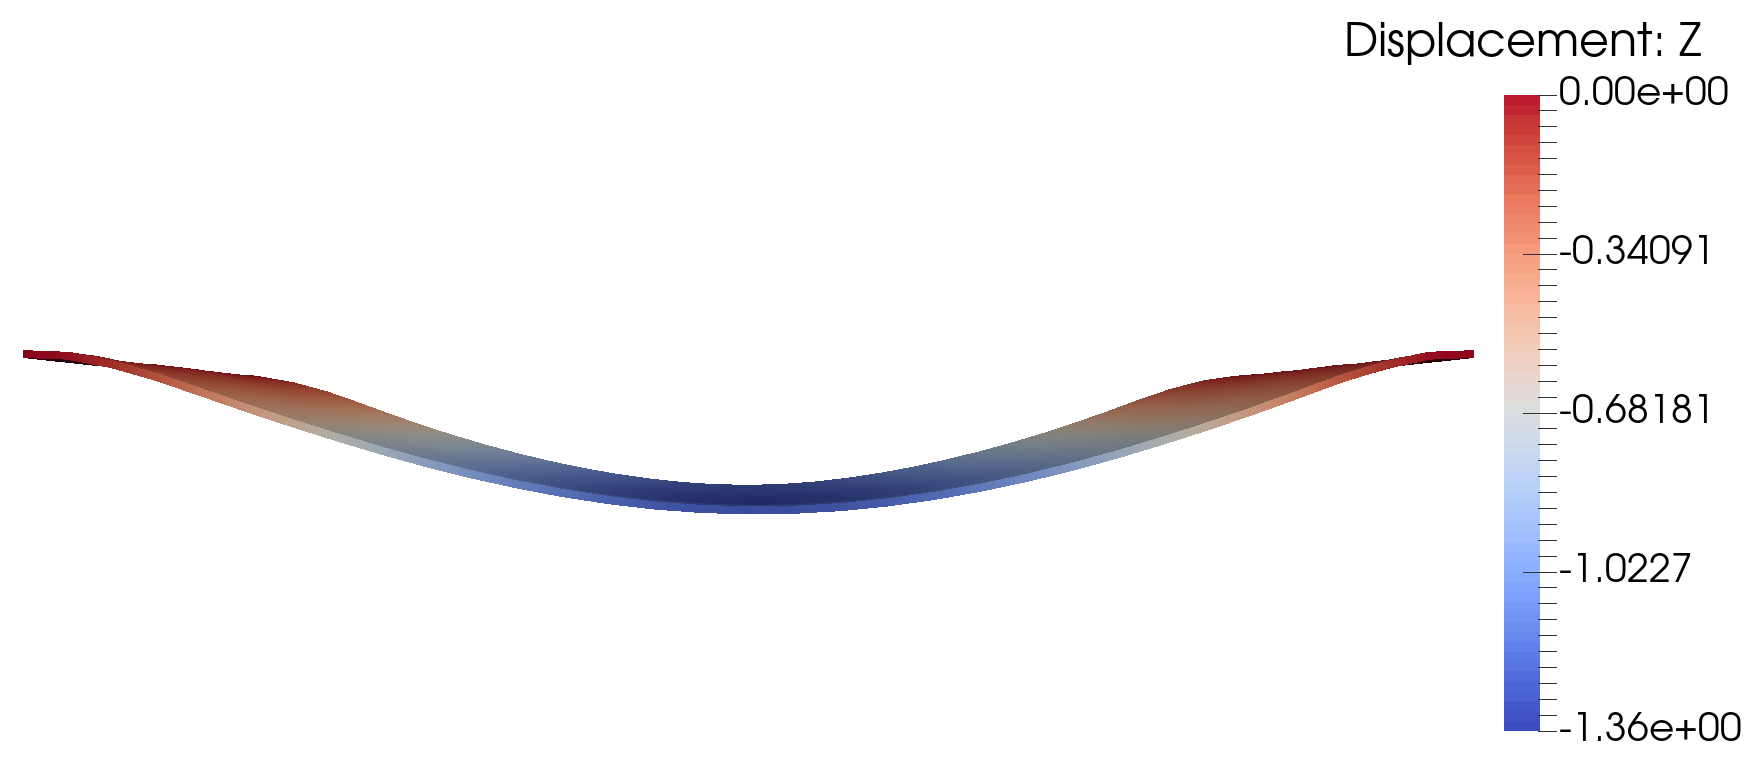
\includegraphics[width=0.85\textwidth, keepaspectratio]
    {panel_side_profile_Z_solution}
  \caption{ Side profile of deformed mesh at 25s with out of plane displacement coloring.
            Deformations are to scale.}
  \label{fig_panel_side_profile_Z_solution}
\end{figure}

\begin{figure}[H] 
  \centering
    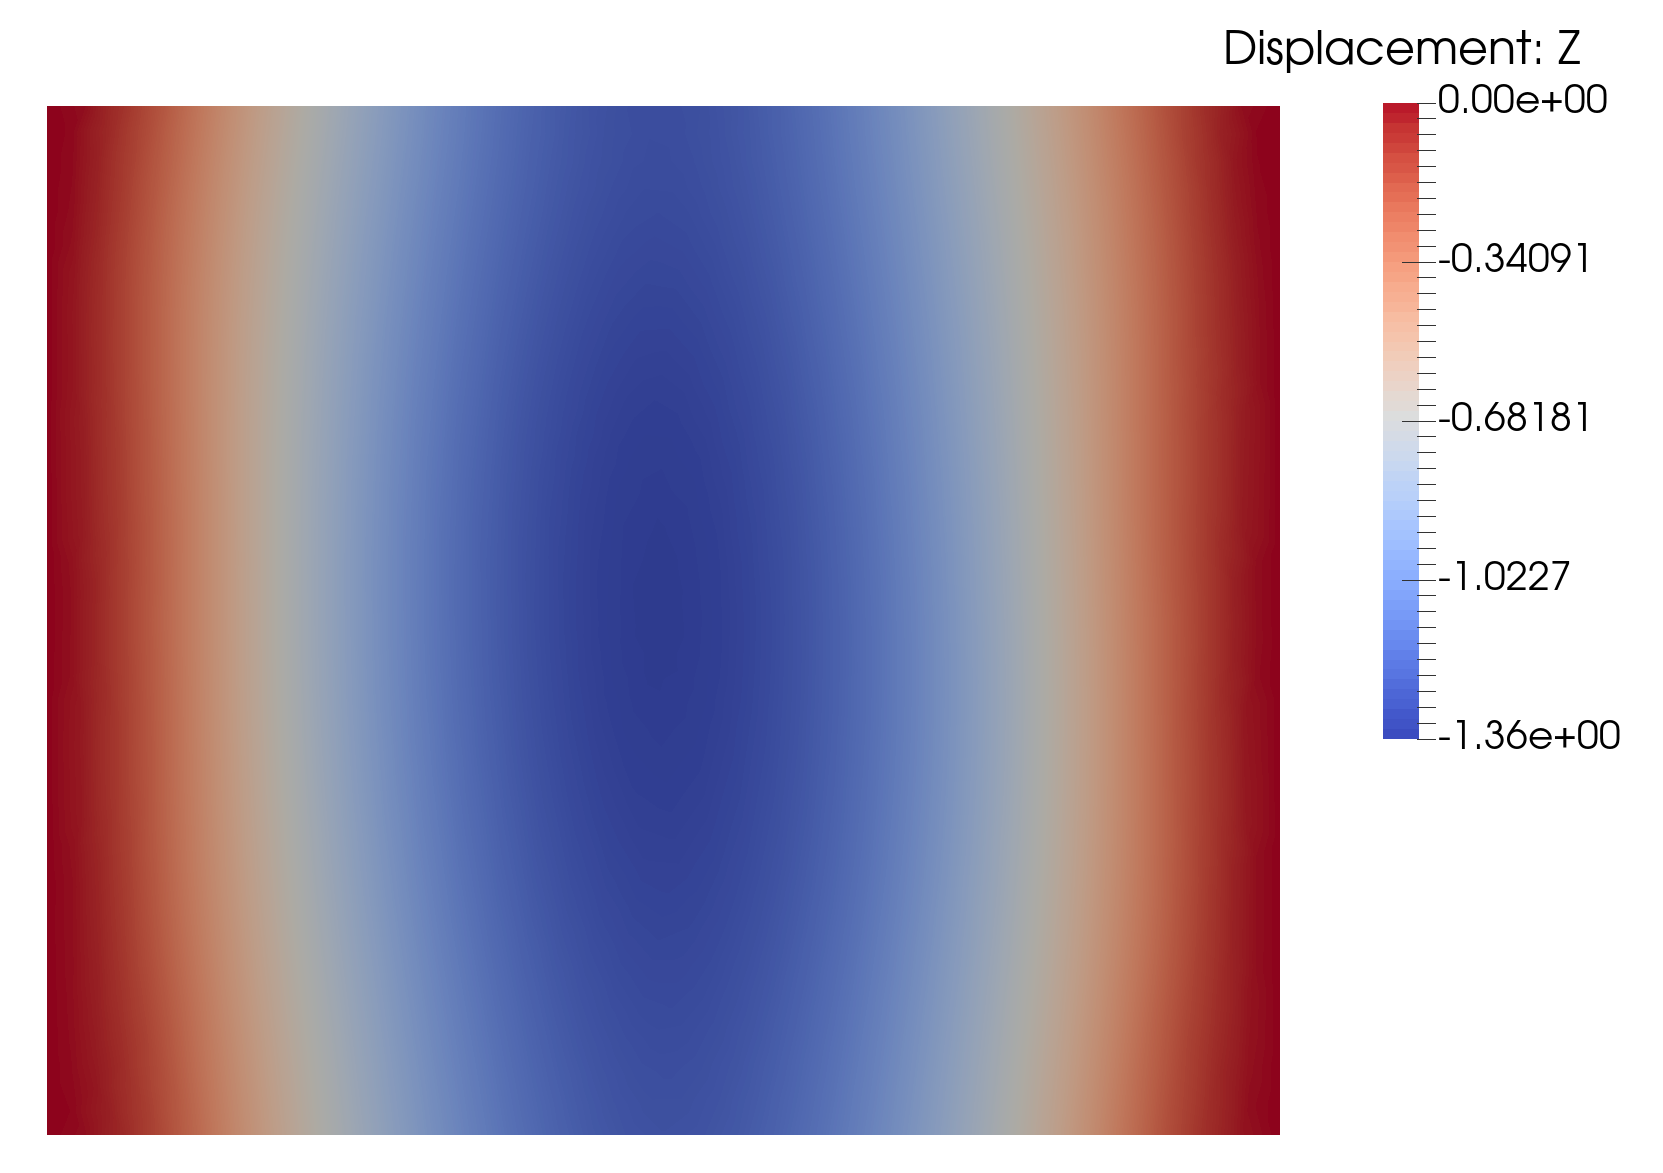
\includegraphics[width=0.85\textwidth, keepaspectratio]
    {panel_top_down_Z_solution}
  \caption{ Panel face at 25s with out of plane displacement coloring.}
  \label{fig_panel_top_down_Z_solution}
\end{figure}

\begin{figure}[H]
  \centering
    \begin{tikzpicture}
      \begin{axis}[
        legend pos=outer north east,
        legend cell align={left},
        grid=both,
        grid style={line width=.1pt, draw=gray!10},
        major grid style={line width=.2pt,draw=gray!50},
        xtick={},
        ytick={},
        yticklabel style={/pgf/number format/.cd, zerofill},
        minor tick num=5,
        xlabel=Time (s),
        title=Out of Plane Displacement at Panel Center Point,
        ylabel={Displacement [in] } 
        ]
        \addplot[black, thick] table {data/panel_solution_Z_over_time.txt};
      \end{axis}
    \end{tikzpicture}
  \caption{ Out of plane displacement over time at center point of panel.}
  \label{fig_panel_displacement_over_time}
\end{figure}

The 1,1 component of the Cauchy stress is plotted with respect to time
for the center point on the face of the panel in Figure \ref{fig_panel_stress_over_time}.
The value of stress is normalized with respect to the reference stress, 
$\sigma_0 = 22.7 \text{MPa}$.

\begin{figure}[H]
  \centering
    \begin{tikzpicture}
      \begin{axis}[
        legend pos=outer north east,
        legend cell align={left},
        grid=both,
        grid style={line width=.1pt, draw=gray!10},
        major grid style={line width=.2pt,draw=gray!50},
        xtick={},
        ytick={},
        yticklabel style={/pgf/number format/.cd, zerofill},
        minor tick num=5,
        xlabel=Time (s),
        title=Stress at Center of Panel Face,
        ylabel={Stress [$\sigma_0$] } 
        ]
        \addplot[black, thick] table {data/panel_stress_over_time.txt};
      \end{axis}
    \end{tikzpicture}
  \caption{ Stress component 1,1 at center point of panel face.}
  \label{fig_panel_stress_over_time}
\end{figure}

The curve plotted in Figure \ref{fig_panel_stress_over_time} first 
shows a sharp increase in compressive stress from zero to 5s.
This is due to the increasing thermal and pressure loads on the panel.
At roughly the 5s mark, the stress begins to decrease. 
This time corresponds to a temperature of 593 K. 
Although this is only 20\% of the 3019 K activation temperature,
the built up stress of 6.82 $\sigma_0$ is sufficient to generate 
inelastic strain through creep.
During the remaining time, from 5s to 25s, the temperature 
and pressure continue to increase but the magnitude of stress in the plate
decreases.

The panel colored with the 1,1 stress component is shown at 5s
and 25s in Figures \ref{fig_panel_stress_5s} and 
\ref{fig_panel_stress_25s}, respectively.
The Frobenius norm at these two times are also shown 
in Figures \ref{fig_panel_stress_frobenius_5s}
and \ref{fig_panel_stress_frobenius_25s}.

\begin{figure}[H] 
  \centering
    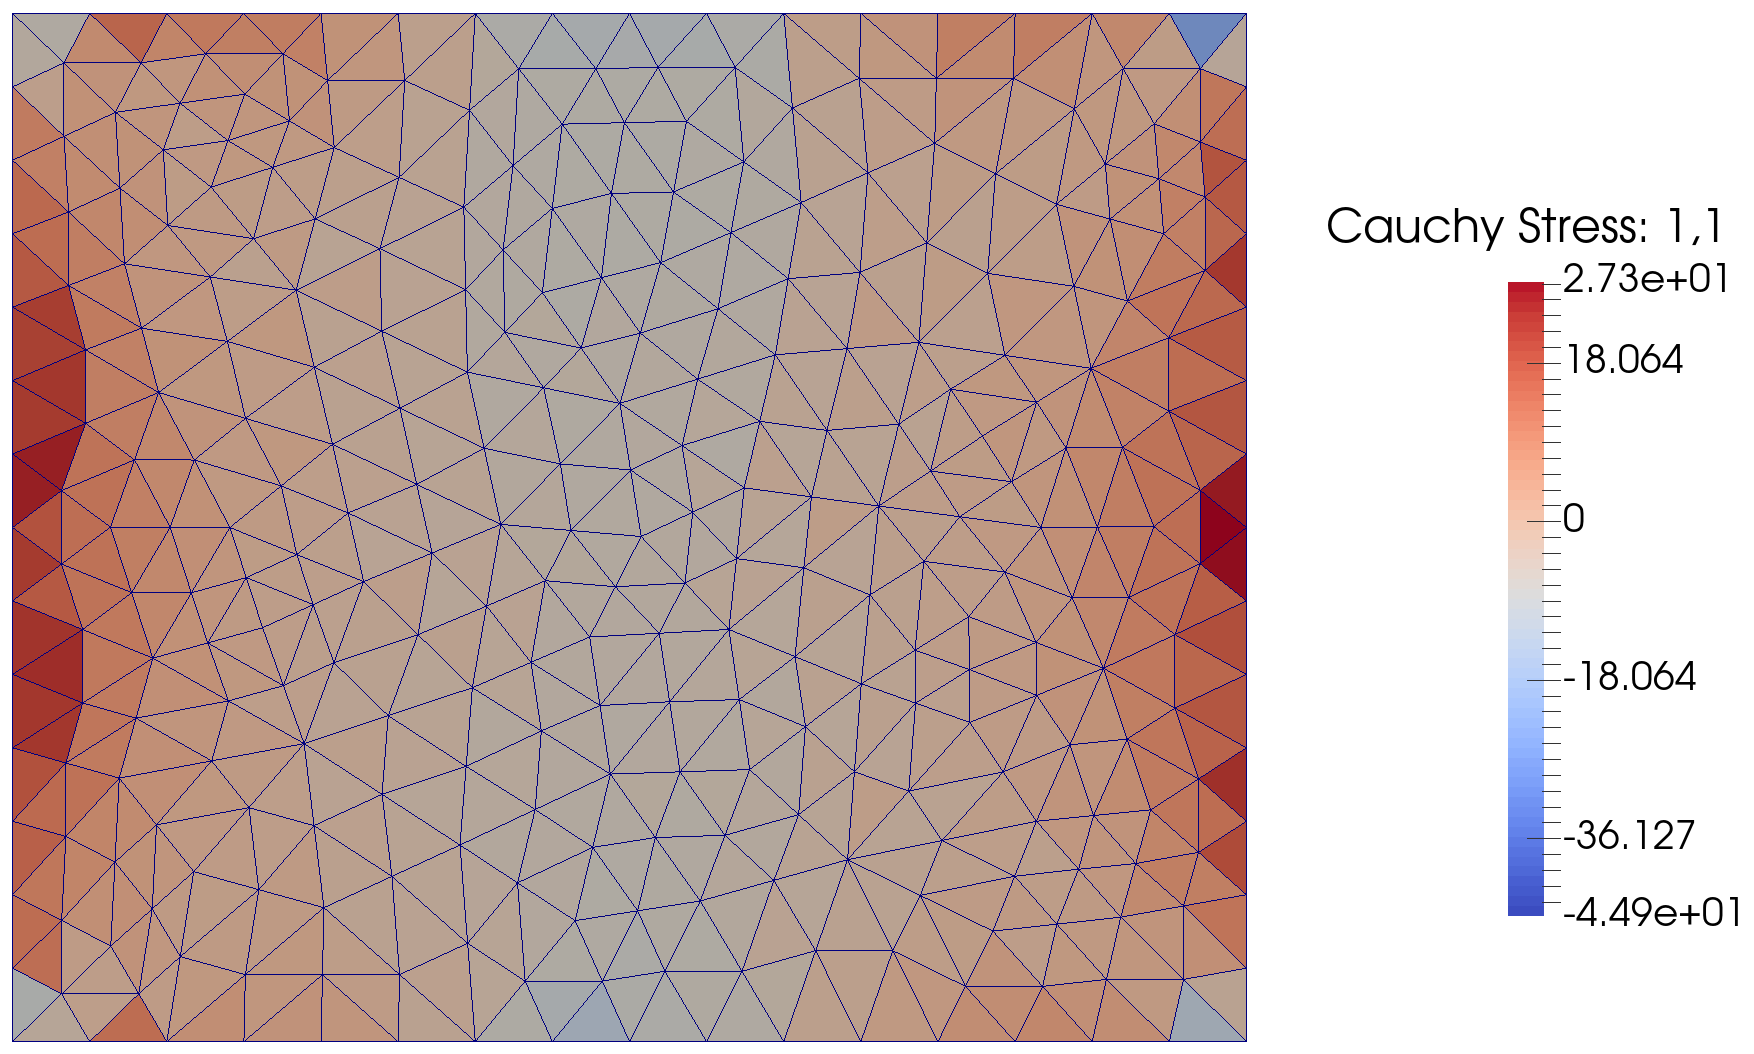
\includegraphics[width=0.85\textwidth, keepaspectratio]
    {panel_stress_5s}
  \caption{ Panel with stress component 1,1 coloring at 5s.
            Stress has units of $\sigma_0$.}
  \label{fig_panel_stress_5s}
\end{figure}

\begin{figure}[H] 
  \centering
    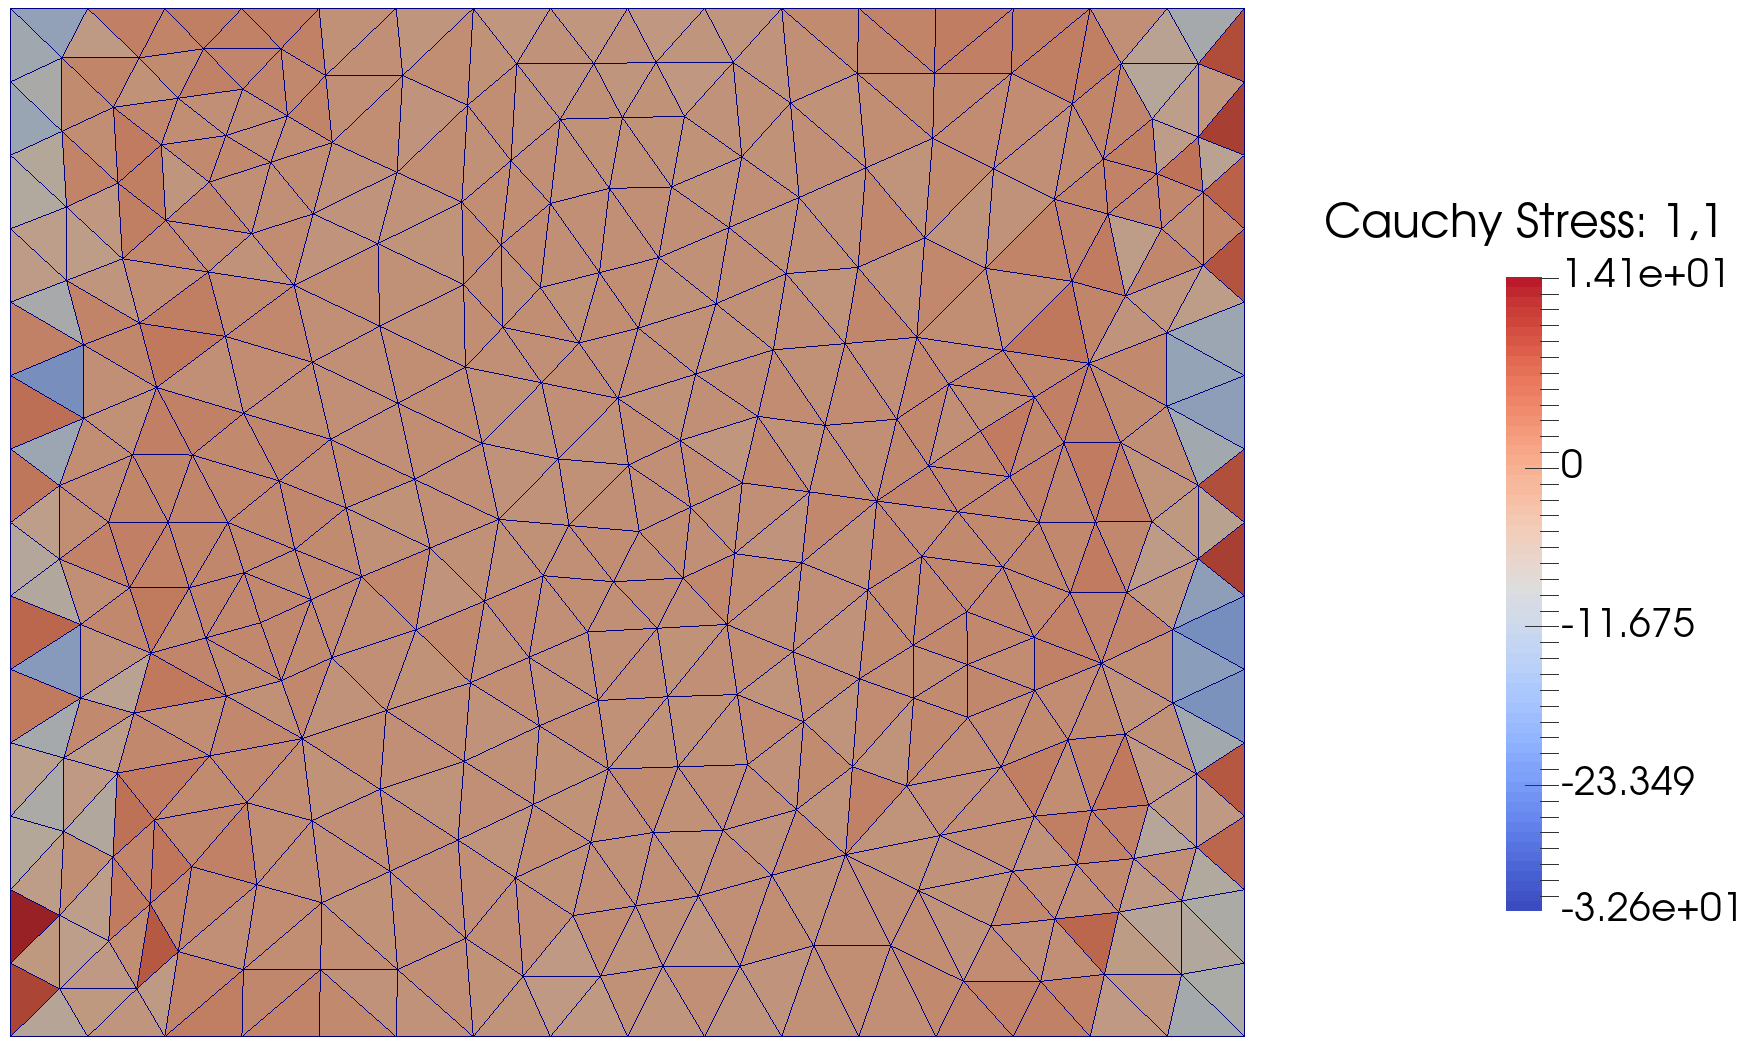
\includegraphics[width=0.85\textwidth, keepaspectratio]
    {panel_stress_25s}
  \caption{ Panel with stress component 1,1 coloring at 25s.
            Stress has units of $\sigma_0$.}
  \label{fig_panel_stress_25s}
\end{figure}

\begin{figure}[H] 
  \centering
    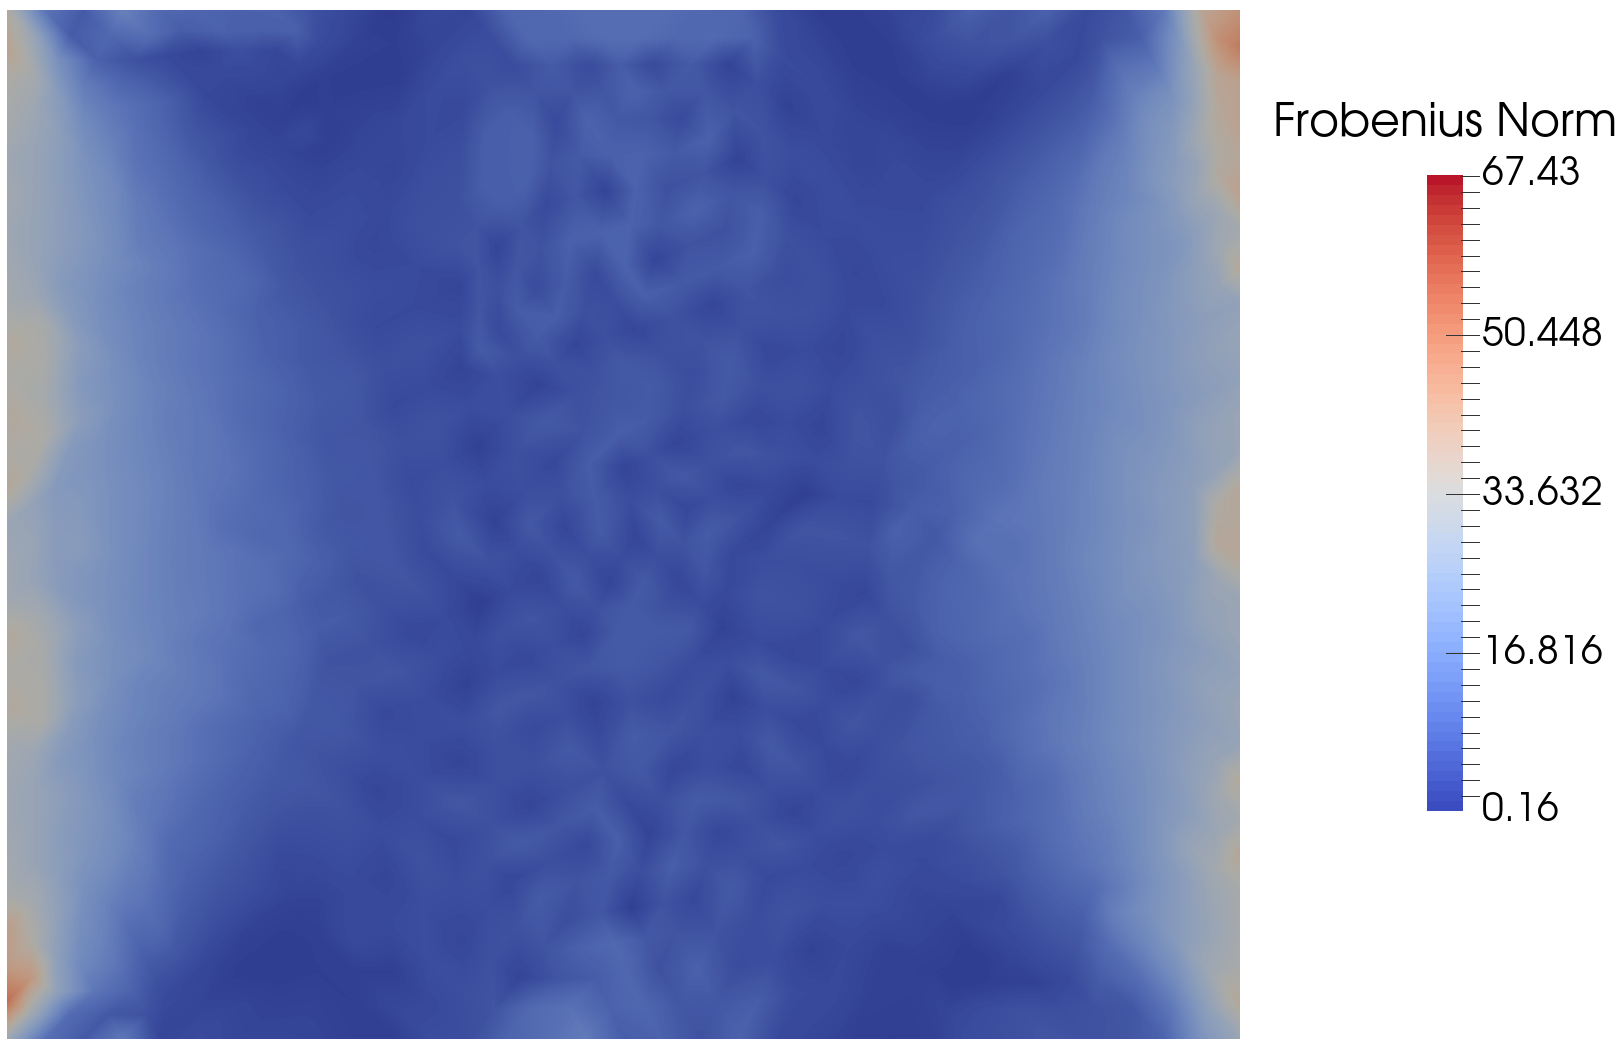
\includegraphics[width=0.85\textwidth, keepaspectratio]
    {panel_stress_frobenius_norm_5s}
  \caption{ Panel with Frobenius norm of stress coloring at 5s.
            Stress has units of $\sigma_0$.}
  \label{fig_panel_stress_frobenius_5s}
\end{figure}

\begin{figure}[H] 
  \centering
    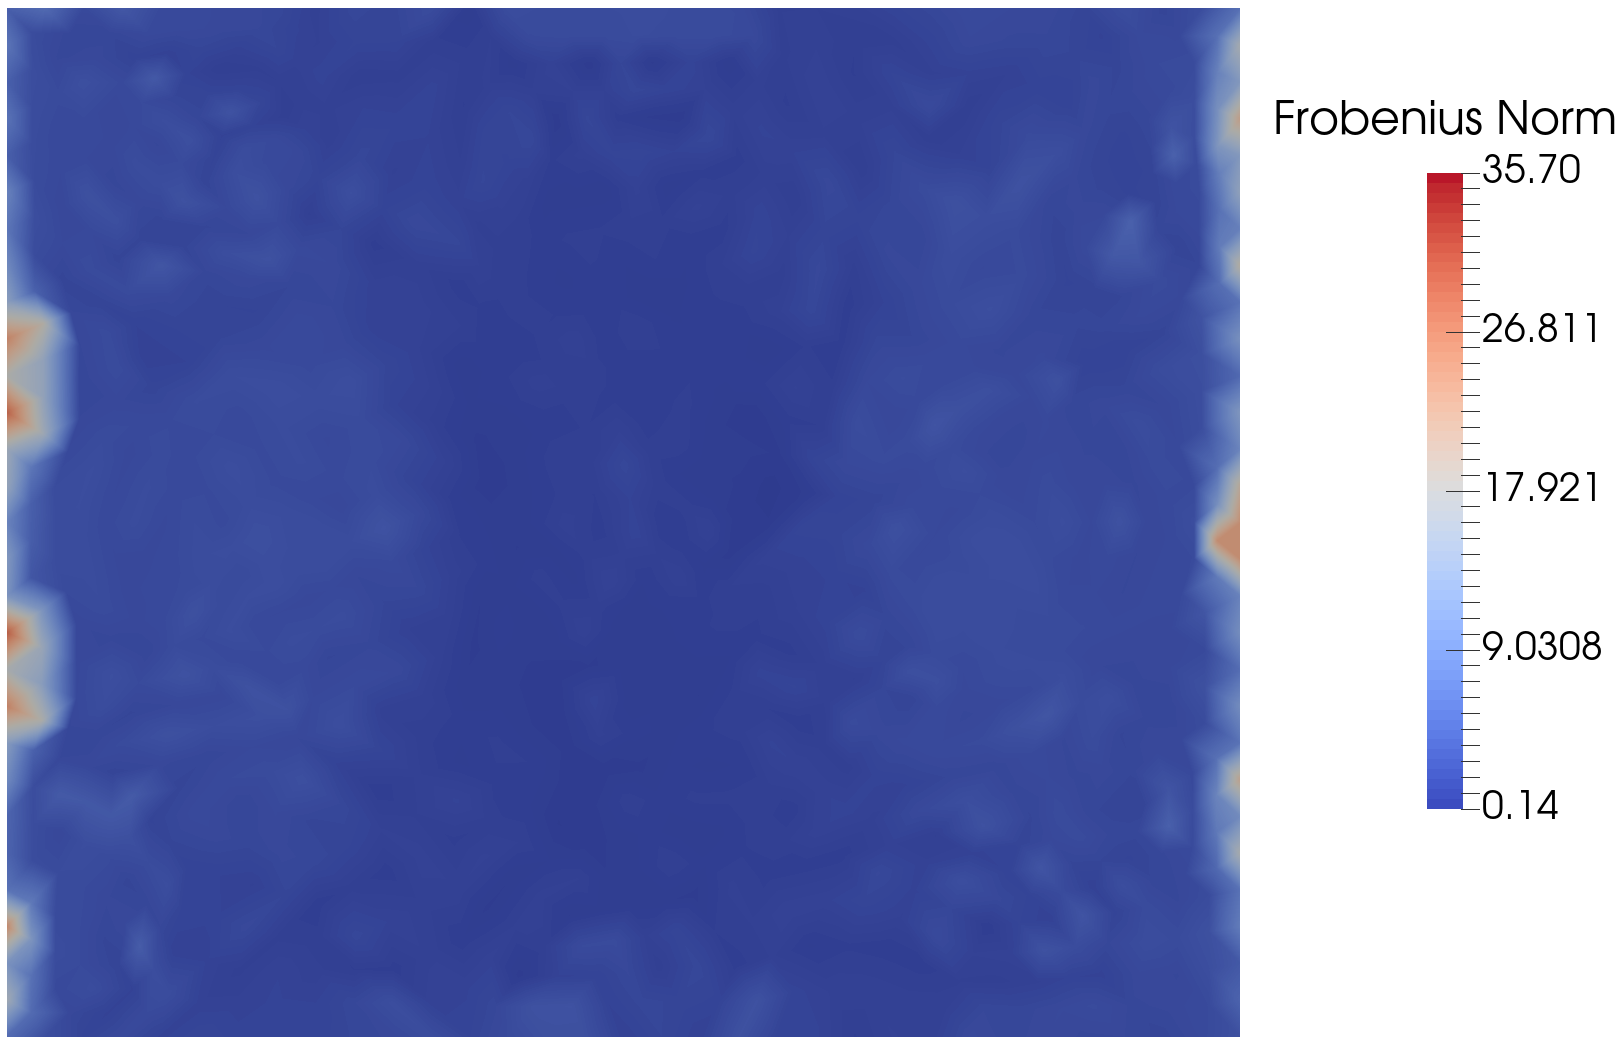
\includegraphics[width=0.85\textwidth, keepaspectratio]
    {panel_stress_forbenius_norm_25s}
  \caption{ Panel with Frobenius norm of stress coloring at 25s.
            Stress has units of $\sigma_0$.}
  \label{fig_panel_stress_frobenius_25s}
\end{figure}

\noindent
The stress contours in Figures \ref{fig_panel_stress_5s} through
\ref{fig_panel_stress_frobenius_25s} show that stress history 
shown in Figure \ref{fig_panel_stress_over_time} is not unique to 
the center point. 
Points throughout the panel first undergo a sharp increase in
the magnitude of stress in the first 5 seconds of heating. 
After that point, the stress reduces even as heating continues to increase.
The decrease in stress is due to the activation of the creep mechanism.
After 5s the ratios of temperature and stress to activation temperature
and reference stress are great enough to cause inelastic strain.
For example, this is shown by the maximum value of the Frobenius norm 
decreasing from $67.43\sigma_0$ at 5s to $35.70\sigma_0$ at 25s.


%-----------------------------------------------------------------------------%
\section{Discussion and Closing Remarks} \label{sec_closing_remarks}

This study's goal was to investigate the importance of creep in typical 
body panels for representative high speed vehicles.
First, a 1D approximation was made using a bar to represent a strip of
paneling. 
The constitutive law was also approximated using an additive strain decomposition
as opposed to a multiplicative one to allow for an analytical solution.
Using flight parameters provided by 
\cite{culler_impact_of_FTS_coupling_on_response_prediction_hypersonic_skin_panels},
it was found that the change in temperature is great
enough to cause large stresses in the bar. 
Those stresses, combined with the high absolute temperature, activated the creep mechanism.
This allows the magnitude of stress within the bar to decreases as inelastic strain increases. 
Once held at a steady temperature, the material finishes relaxing and holds 
its new stress state. 
When the bar was then cooled, there was less than a 1\% change in the inelastic strain
whereas the magnitude of stress increased. 
After a second heating phase, the stress in the bar relaxed again. 

Similar results were found with a slower heating and cooling time.
However, during the slower cooling phase, the inelastic strain initially decreased in magnitude.
This is due to the lowering temperature difference causing the bar to contract,
yet the absolute temperature was still great enough to allow creep to occur. 
Once the absolute temperature fell below the threshold, creep relaxation 
stopped; this caused the inelastic strain to stagnate and the stress to increase
in magnitude. 

The full panel exhibited similar behavior during the investigate heating phase.
Initially, a sharp increase of the magnitude of stress is observed.
This is due to the increasing temperature and pressure causing the panel
to deform into the plane; 
this large deformation then corresponded to a large stress buildup.
At 5s, the stress in the panel then begins to relax due to creep.
This trend holds for the rest of the simulated time as the temperature and 
pressure continue to increase. 
Similar behavior during cooling and reheating to the 1D bar approximation 
is expected from the full panel. 
Namely, some inelastic strain decrease during cooling and subsequent 
increase during reheating as well as an increase in stress during cooling
and decrease during reheating.

The models show two main points:
\begin{itemize}
  \item The creep mechanism is active during canonical high speed 
    vehicle flights. Temperatures and stresses are great enough to 
    cause stress relaxation through creep.
  \item Inelastic strain is generated during the heating phase
    of flight cycles and is not fully eliminated during the cooling phase.
\end{itemize}
Together, the above two points also indicate that significant residual 
stresses remain in the panel after cooling. 
Although plasticity through the $J_2$ flow rule was not considered 
in this study, the residual stresses predicted by the 1D bar 
are greater than the material's yield stress. 
If modeled, this would also be a source of inelastic strain.
Both sources of inelastic strain would not appear uniformly
throughout the panel which could lead to other effects 
during repeated flights.

%-----------------------------------------------------------------------------%
\section{Future Work} \label{sec_future}
future work text

This preliminary work shows that the creep mechanism plays 
an active role in the deformation of high speed panels in flight.
Additional work to be completed includes the following items:

\begin{itemize}
  \item Create a geometric estimation and discretization of a high speed panel.
        A geometry based on the one used in 
        \cite{ culler_impact_of_FTS_coupling_on_response_prediction_hypersonic_skin_panels}
        will be used in this study.
  \item Evaluate the panel using the creep and plasticity model and implementation presented in
        \cite{ li_simulation_of_finite_strain_inelastic_phenomena_governed_by_creep_and_plasticity}.
        A temperature history from 
        \cite{ culler_impact_of_FTS_coupling_on_response_prediction_hypersonic_skin_panels}
        will be prescribed throughout the panel. 
        Multiple flight cycles of heating, cruise, and cooling will be used
        to match historical and conceptual vehicles outlined in
        \cite{ kordes_structureal_heating_experiencs_on_the_x15_airplane,
               zuchowski_AVIATR_Predictive_capability_for_hypersonic_structural_response_and_life_prediction_phase_II}.
  \item Compare the deformation and permanent set of the panel to that 
        found by \cite{ culler_impact_of_FTS_coupling_on_response_prediction_hypersonic_skin_panels}.
\end{itemize}

\noindent
The post-analysis and results will include plots the maximum creep strain, norms of stress, 
and deflection throughout the panel and at points of interest over time. 
Contour plots will also be made showing the total strain, stresses, and deflections
of the panel at key points in time.
Following discussions include the importance of creep 
with respect to other permanent deformation mechanism 
in the high speed flight environment.

%-----------------------------------------------------------------------------%
\section*{Acknowledgments}
The authors thank the DoD Science, Mathematics, And 
Research for Transformation (SMART) Scholarship
for Service Program which sponsored this work.

\bibliography{monolith.bib}

\end{document}
